\chapter{RESULTS}
% TODO: add chapter overview

% write first; keep notes/comments in discussion

% TODO: clinical covariates, clinical information? maybe in appendix...
% TODO: show subtype distribution histogram; or maybe its redundant because its shown in the table below

\section{Cohort Characteristics}

%TODO: refer to methods for dataset retrieval method.. cant think of suitable phrasing rn

TCGA-LUSC datasets for five modalities were retrieved (described in Section~\ref{subsec:data_acquisition}). 

Gene expression and \gls{cnv} retained the full labelled 178-sample cohort, whereas \gls{dna} methylation and miRNA expression had smaller assay overlap (Table~\ref{tab:omics_summary}). Across modalities, the classical subtype was the most frequent class and primitive the least frequent, motivating the use of macro-averaged classification metrics in subsequent analyses.

\begin{table}[H]
\footnotesize
\caption[Summary of omics modalities used in this study]{Summary of omics modalities used in this study. Variation in sample size reflects assay availability and label overlap.}
\centering
\setlength{\tabcolsep}{3pt}
\begin{tabular}{lcccccc}
    \toprule
    \textbf{Modality} & \textbf{Configuration} & \textbf{Classical} & \textbf{Basal} & \textbf{Secretory} & \textbf{Primitive} & \textbf{Total} \\
    \midrule
    Gene expression & HiSeqV2, RNASeqV2 RSEM-normalised & 65 & 43 & 43 & 27  & 178 \\
    DNA methylation & HumanMethylation450k beta values & 29 & 14 & 22 & 11  & 76 \\
    miRNA expression & miRNA sequencing, log2(RPM + 1) & 44 & 29 & 20 & 14  & 107 \\
    RPPA & Normalised protein abundance & 38 & 28 & 28 & 18 & 112 \\
    CNV & GISTIC2 all-thresholded calls & 65 & 43 & 43 & 27 & 178 \\
    \bottomrule
\end{tabular}
\label{tab:omics_summary}
\end{table}

\section{Preprocessing Summary}

\begin{figure}[H]
\centering
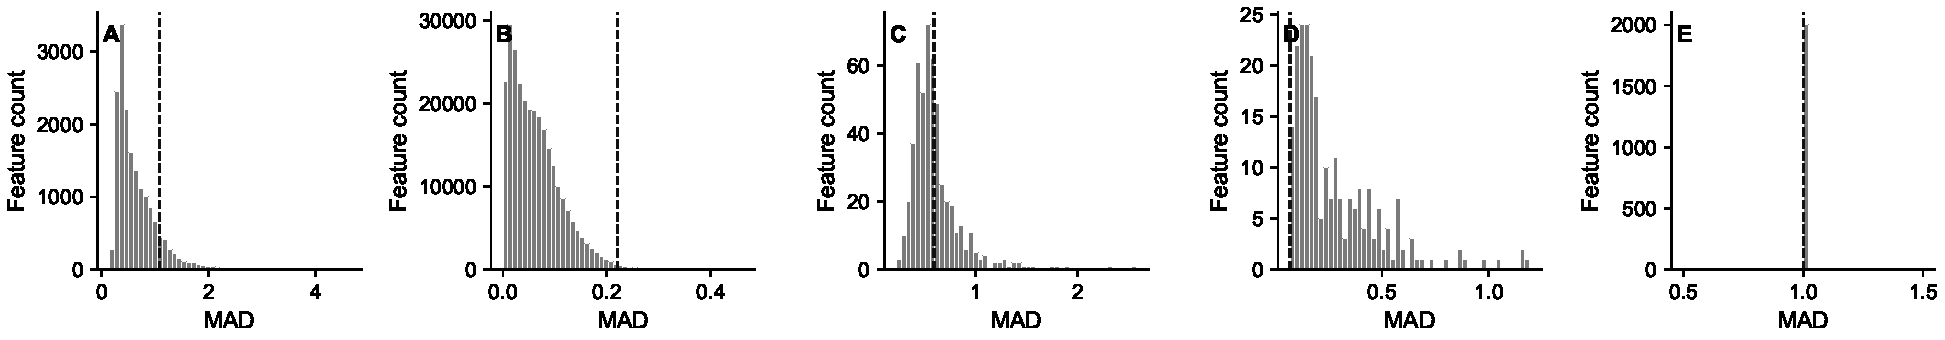
\includegraphics[width=\textwidth]{figures/eda/feature_variability_distributions.pdf}
\caption[Feature variability distributions across omics modalities]{Feature variability distribution across processed omics modalities. Panels show MAD distributions for (A) gene expression, (B) \gls{dna} methylation, (C) \gls{mirna} expression, (D) RPPA, and (E) \gls{cnv}. Dashed vertical lines denote retained-feature threshold used for the processed matrix; for RPPA, all 238 antibodies were retained and the line denotes the minimum retained MAD.}
\label{fig:eda_feature_variability}
\end{figure}


\begin{table}[H]    
\footnotesize
\centering
\caption[Preprocessing and feature-retention summary]{Preprocessing and feature-retention summary for each omics modality. Raw feature counts correspond to the input assay feature spaces. The MAD threshold is the score of the last retained feature in the processed matrix; for RPPA, where all 238 antibodies were retained, this value represents the minimum observed MAD among retained antibodies.}
\begin{tabular}{lccc}
    \toprule
    \textbf{Modality} & \textbf{Raw features} & \textbf{Retained features} & \textbf{MAD threshold} \\
    \midrule
    Gene expression & 60,660 & 2,000 & 1.0808 \\
    \gls{dna} methylation & 485,577 & 2,000 & 0.2208 \\
    \gls{mirna} expression & 1,881 & 200 & 0.5954 \\
    RPPA & 238 & 238 & 0.0692 \\
    \gls{cnv} & 24,776 & 2,000 & 1.0000 \\
    \bottomrule
\end{tabular}
\label{tab:eda_preprocessing_summary}
\end{table}


\begin{figure}[H]
\centering
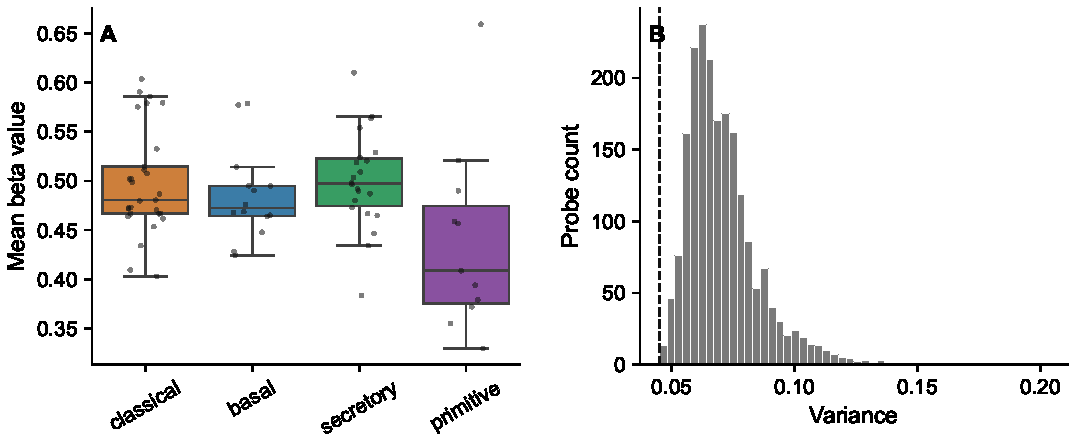
\includegraphics[width=0.82\textwidth]{figures/eda/methylation_mean_beta_and_variance.pdf}
\caption[Methylation beta values and retained-probe variance]{\gls{dna} methylation overview for labelled samples. (A) Mean beta value per sample stratified by subtype. Boxplots show median and interquartile range; points show individual samples. (B) Variance distribution across retained methylation probes. Dashed line denotes the minimum variance among retained probes in the processed matrix.}
\label{fig:eda_methylation}
\end{figure}


% TODO: i need mirna annotations; mirbase server/ftp seems down; might have to check for raw annotations
\begin{figure}[H]
\centering
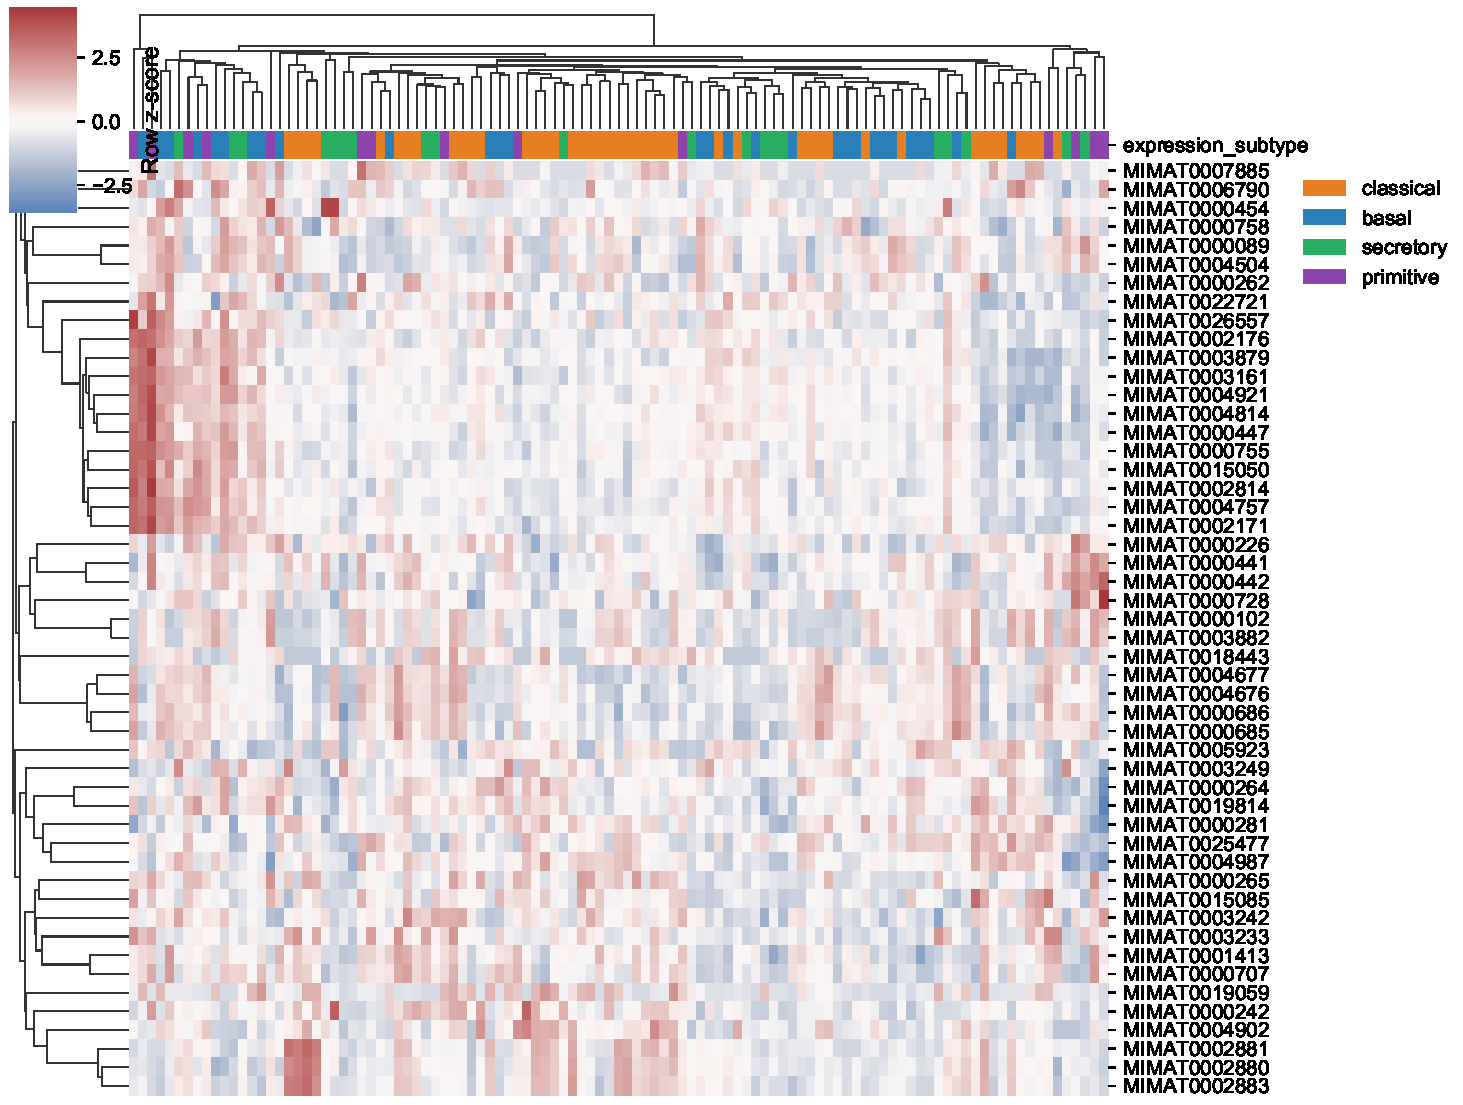
\includegraphics[width=0.88\textwidth]{figures/eda/mirna_top50_variable_heatmap.pdf}
\caption[Top variable miRNA heatmap]{Clustered heatmap of 50 most variable \gls{mirna} features across labelled \gls{tcga}-\gls{lusc} samples. Rows are \gls{mirna} features and columns are samples; values are row-scaled z-scores.}
\label{fig:eda_mirna_heatmap}
\end{figure}

\begin{figure}[H]
\centering
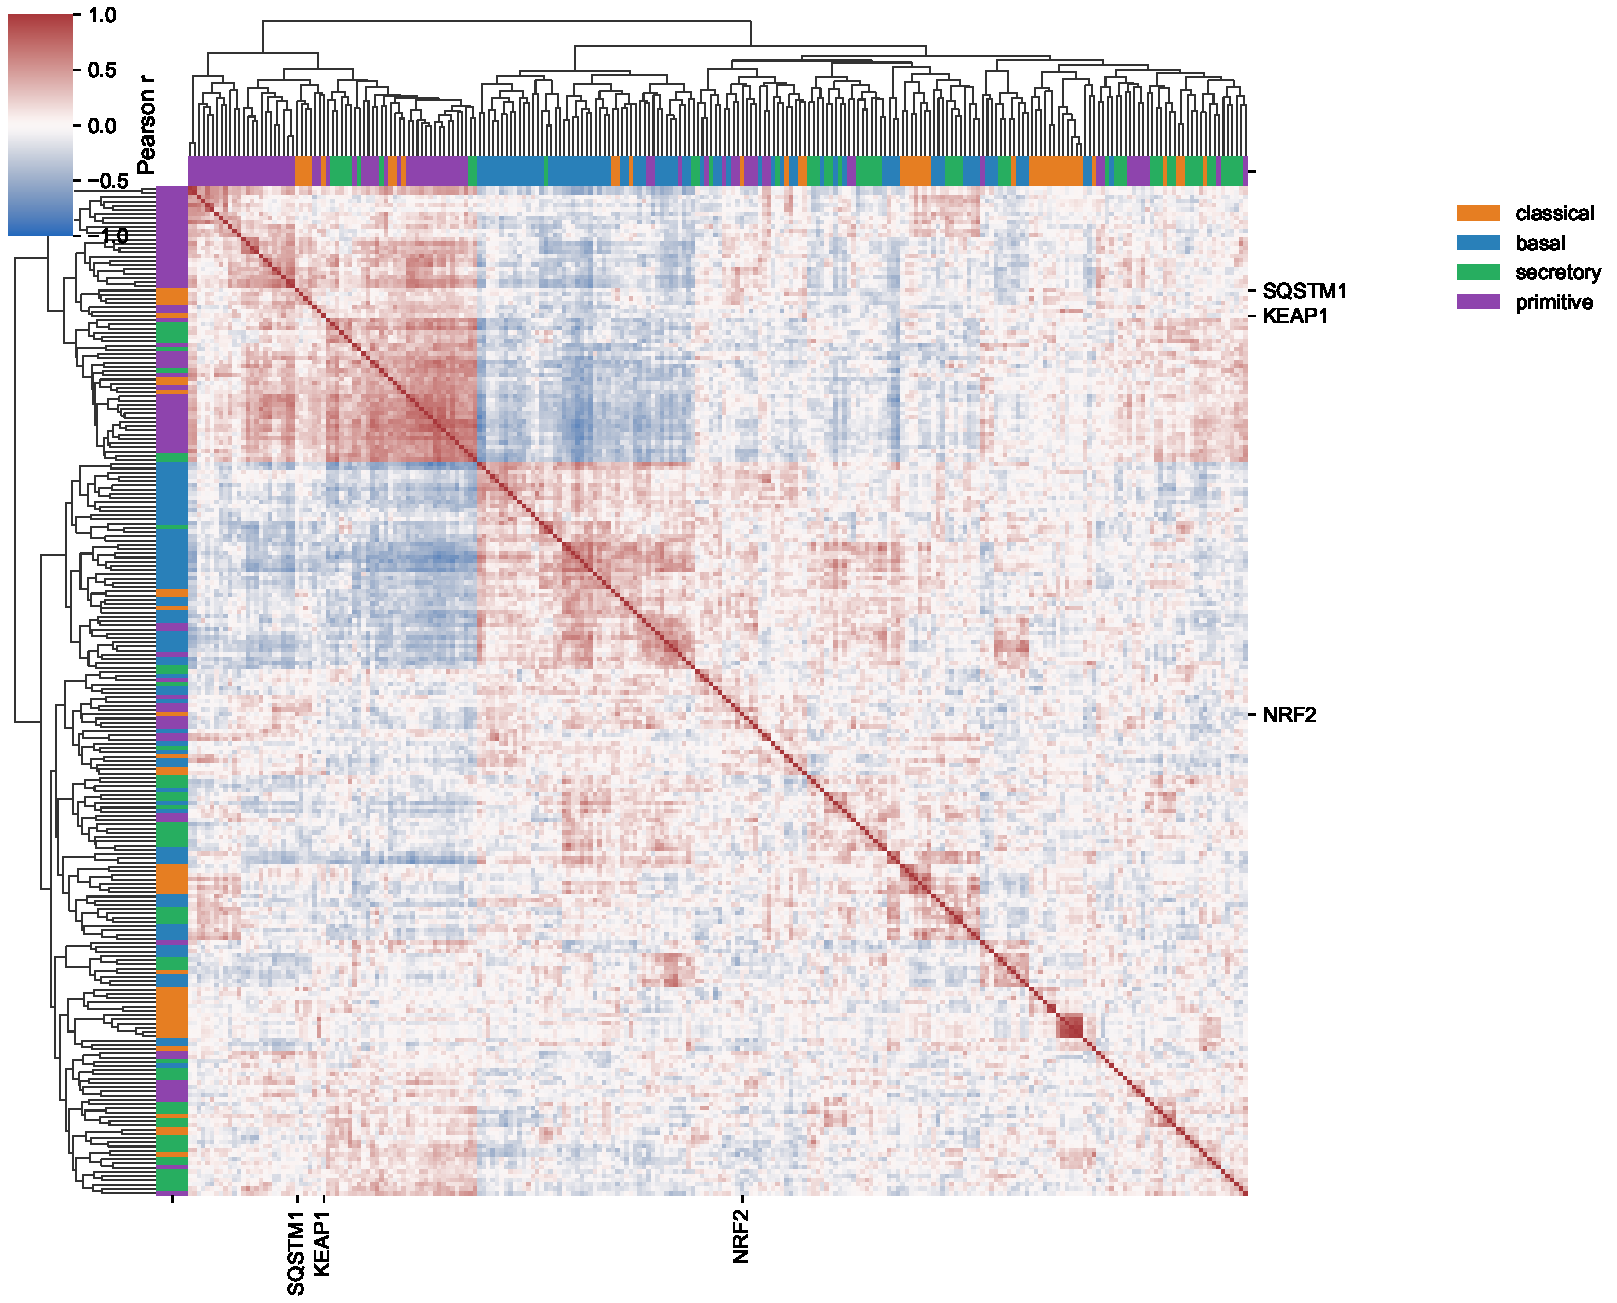
\includegraphics[width=0.90\textwidth]{figures/eda/rppa_antibody_correlation_heatmap.pdf}
\caption[RPPA antibody correlation heatmap]{Hierarchically-clustered correlation heatmap across all 238 RPPA antibodies. Rows and columns represent antibodies, and colour denotes antibody-antibody correlation across RPPA samples. The top and side annotation strips indicate the expression subtype in which each antibody had the highest mean abundance. }
\label{fig:eda_rppa_correlation}
\end{figure}

\begin{figure}[H]
\centering
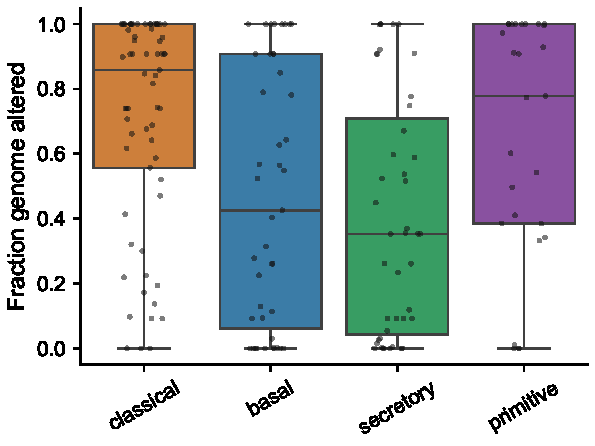
\includegraphics[width=0.56\textwidth]{figures/eda/cnv_fraction_genome_altered.pdf}
\caption[CNV fraction genome altered by subtype]{Fraction of retained \gls{cnv} features with non-zero GISTIC2-thresholded copy-number state per sample, stratified by subtype. Boxplots show median and interquartile range; points show individual samples. Because the calculation is based on the 2,000 retained \gls{cnv} features, it represents relative alteration burden within the processed \gls{cnv} matrix.}
\label{fig:eda_cnv_fga}
\end{figure}

% argument: lusc subtypes have distinct clinical and biological properties, establishing clinical relevance of classification target, checking if subtype-sp signal exists in data.. 
\section{Characterization of LUSC Subtypes}

\subsection{Clinical Characteristics}
\label{subsec:clinical_characteristics}

% survival curves (OS + PFI primary) os = clinical standard, pfi because tcga-cdr expl. recommends that for lusc; i think two figures side by side makes sense, aes: might have to make the font slightly bigger, for future me

%TODO: keep global log-rank test for both; bh-corrected pairwise table and cox hr table for os; not sure about forest plot for os.

%TODO: cite wilkerson, hammerman for known poorly diff. biology
%TODO: add median survival and 95% CI to fig caption; not happy with caption phrasing rn, will fix later
%TODO: keep pfi as primary endpoint for lusc, in literature; cite liu et al 2018

\begin{figure}[H]
\centering

\begin{subfigure}{0.45\textwidth}
\centering
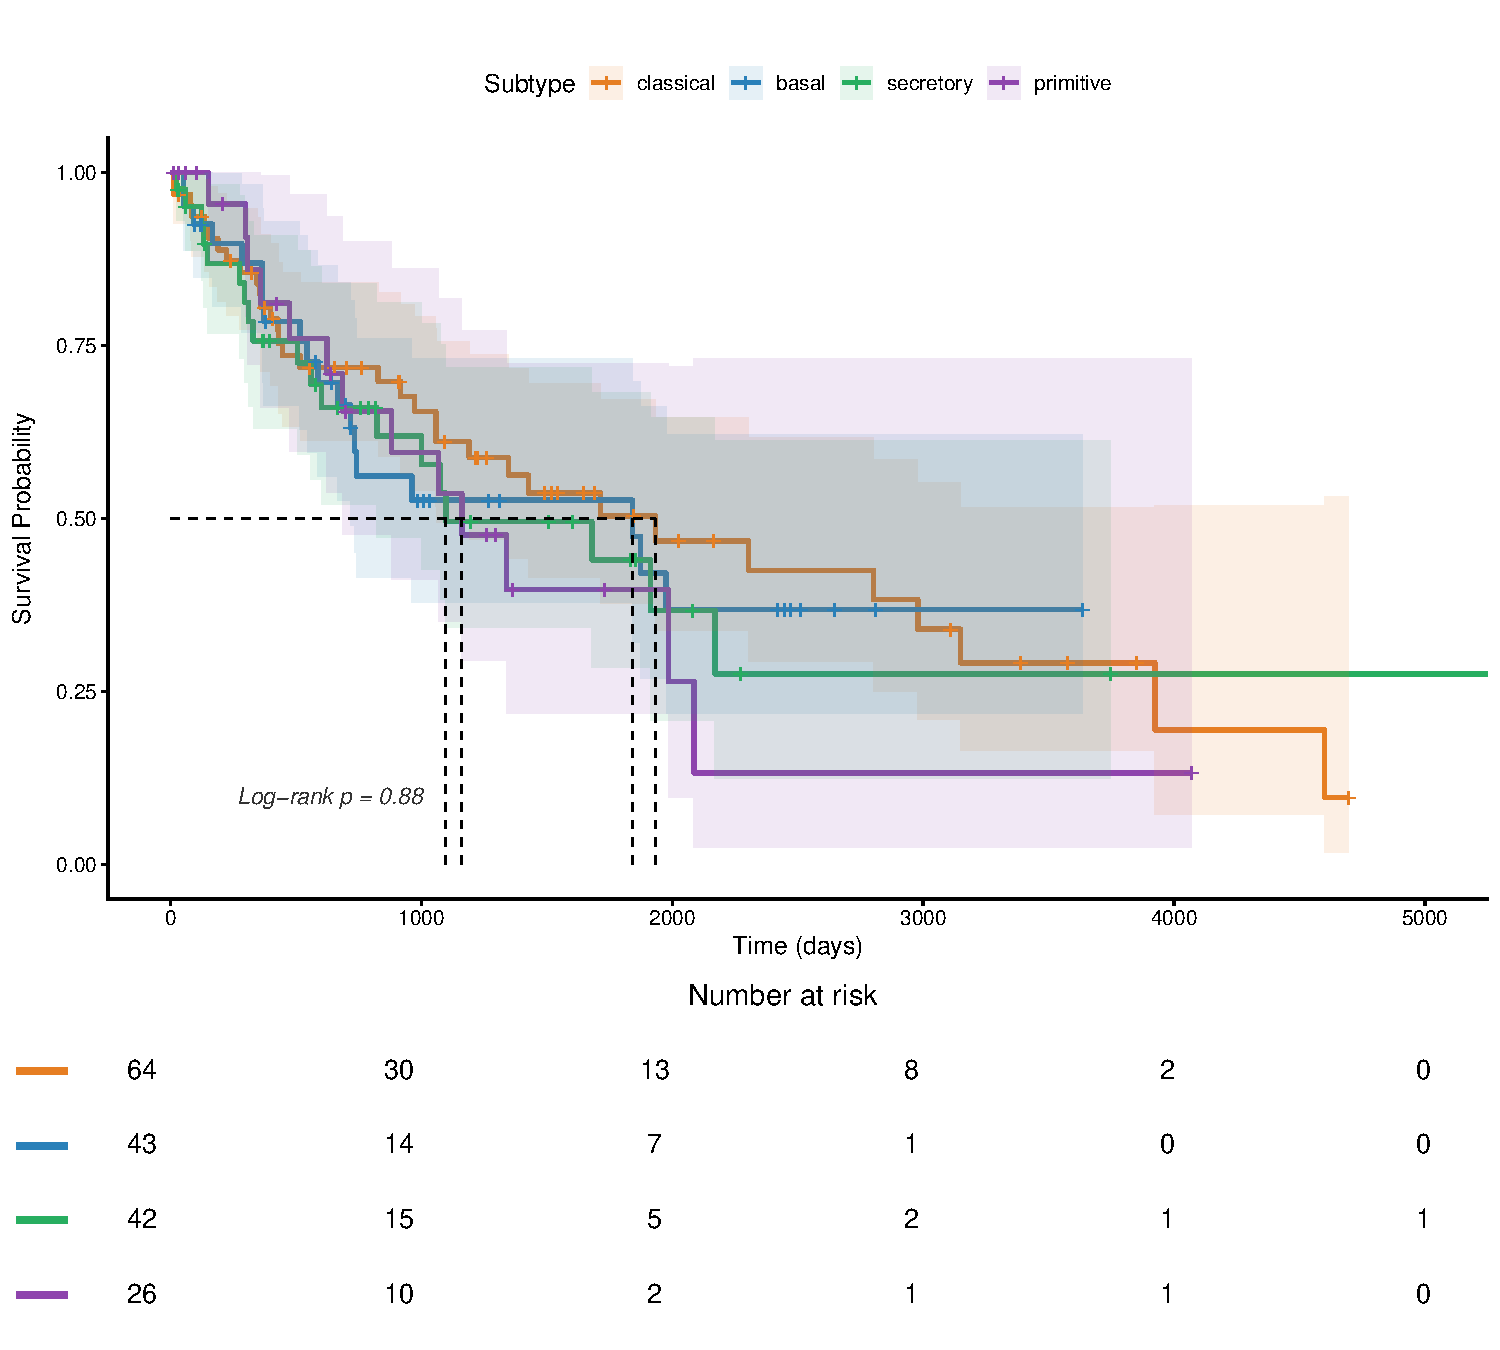
\includegraphics[width=\textwidth]{figures/survival/KM_OS_by_subtype.pdf}
\caption{Overall Survival}
\label{sub:overall_survival}
\end{subfigure}\hspace{0.05\textwidth}
\begin{subfigure}{0.45\textwidth}
\centering
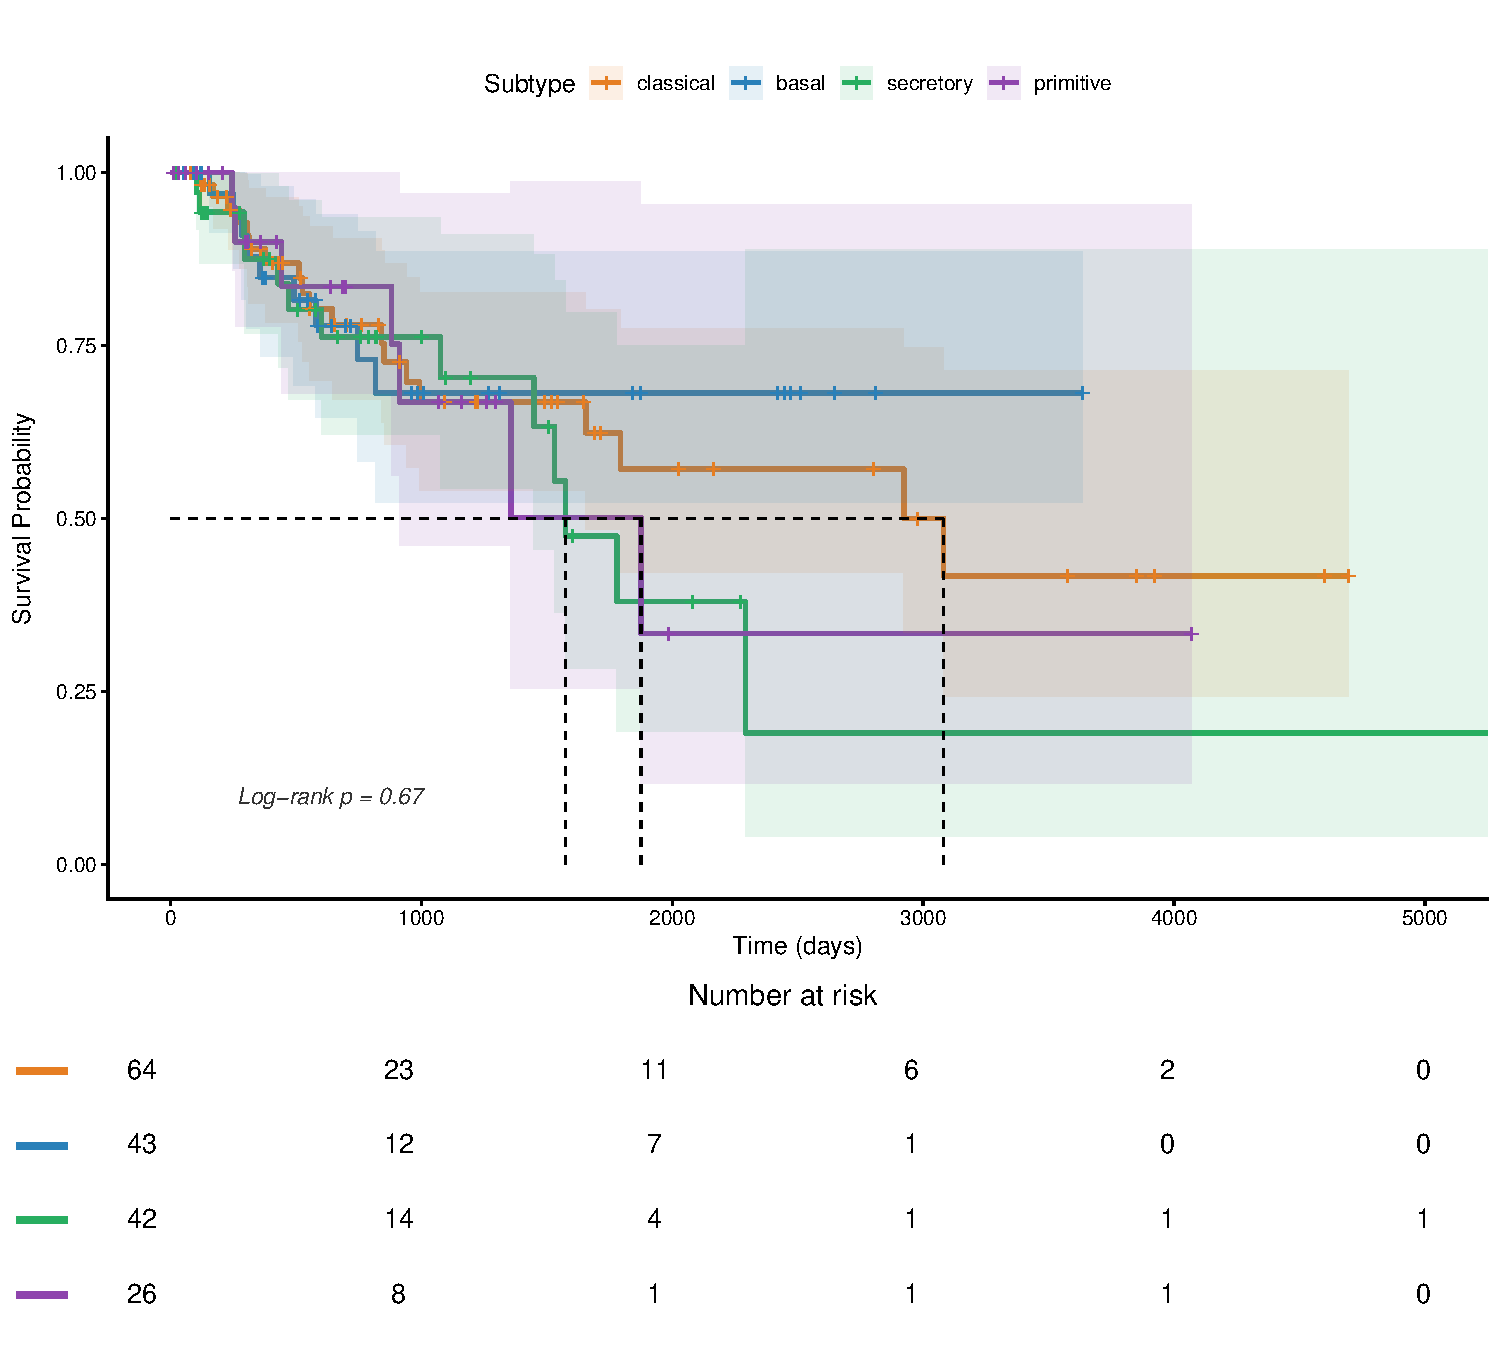
\includegraphics[width=\textwidth]{figures/survival/KM_PFI_by_subtype.pdf}
\caption{Progression-Free Interval}
\label{sub:progression_free}
\end{subfigure}
\caption[KM survival curves for TCGA-LUSC samples stratified by molecular subtypes]{Survival curves showing Overall Survival~(\subref{sub:overall_survival}) and Progression-Free Interval~(\subref{sub:progression_free}) for TCGA-LUSC samples (n=178) stratified by molecular subtypes. Median survival and 95\% confidence intervals were computed by the Brookmeyer-Crowley method. Shaded regions denote 95\% confidence intervals and risk table shows at-risk patient counts at selected time points.}
\label{fig:km_survival_by_subtype}
\end{figure}

Secretory and primitive subtype show the shortest median OS of 36 months and 38.1 months respectively, consistent with known proliferative and poorly differentiated biology of primitive subtypes \parencite{Wilkerson2010,Hammerman2012}.

%TODO: fill placeholder values; marked AVOCADO in red from my r notebooks
%do i really need schoenfeld residuals here? not the focus of main body; maybe move this to appendix.
\begin{figure}[H]
\centering
\includegraphics[width=0.45\textwidth]{figures/survival/forest_plot_os.pdf}
\caption[Forest plot, Cox PH model for OS]{Hazard ratios for overall survival by LUSC molecular subtype from Cox proportional hazards regression, with classical subtype as reference (n=\textcolor{red}{AVOCADO}). Points denote hazard ratios and horizontal bars represent 95\% confidence intervals. HR $>$ 1 indicates worse prognosis relative to classical subtype. The proportional hazards assumption was verified using scaled Schoenfeld residuals (cox.zph global p=\textcolor{red}{AVOCADO}). Concordance index=\textcolor{red}{AVOCADO}}
\label{fig:forest_plot_os}
\end{figure}

\subsection{Immune Microenvironment} %epic, xcell, mcpcounter; maybe cibersort if they approve my req in time
\label{subsec:immune_microenvironment}

% TODO: check nature COMPASS paper that came out recently; uses bulk expression for immune response; could be interesting.
% partly to check if the cohorts show expected immune profile..
% cibersort removed from original plan; cibersort isnt suggested by sturm2019; epic+xcell = better idea for now; suggests picking method per cell type but considering epic,xcell as comparing would be harder if i used a separate tool for every cell type.


\begin{figure}[H]
    \centering
    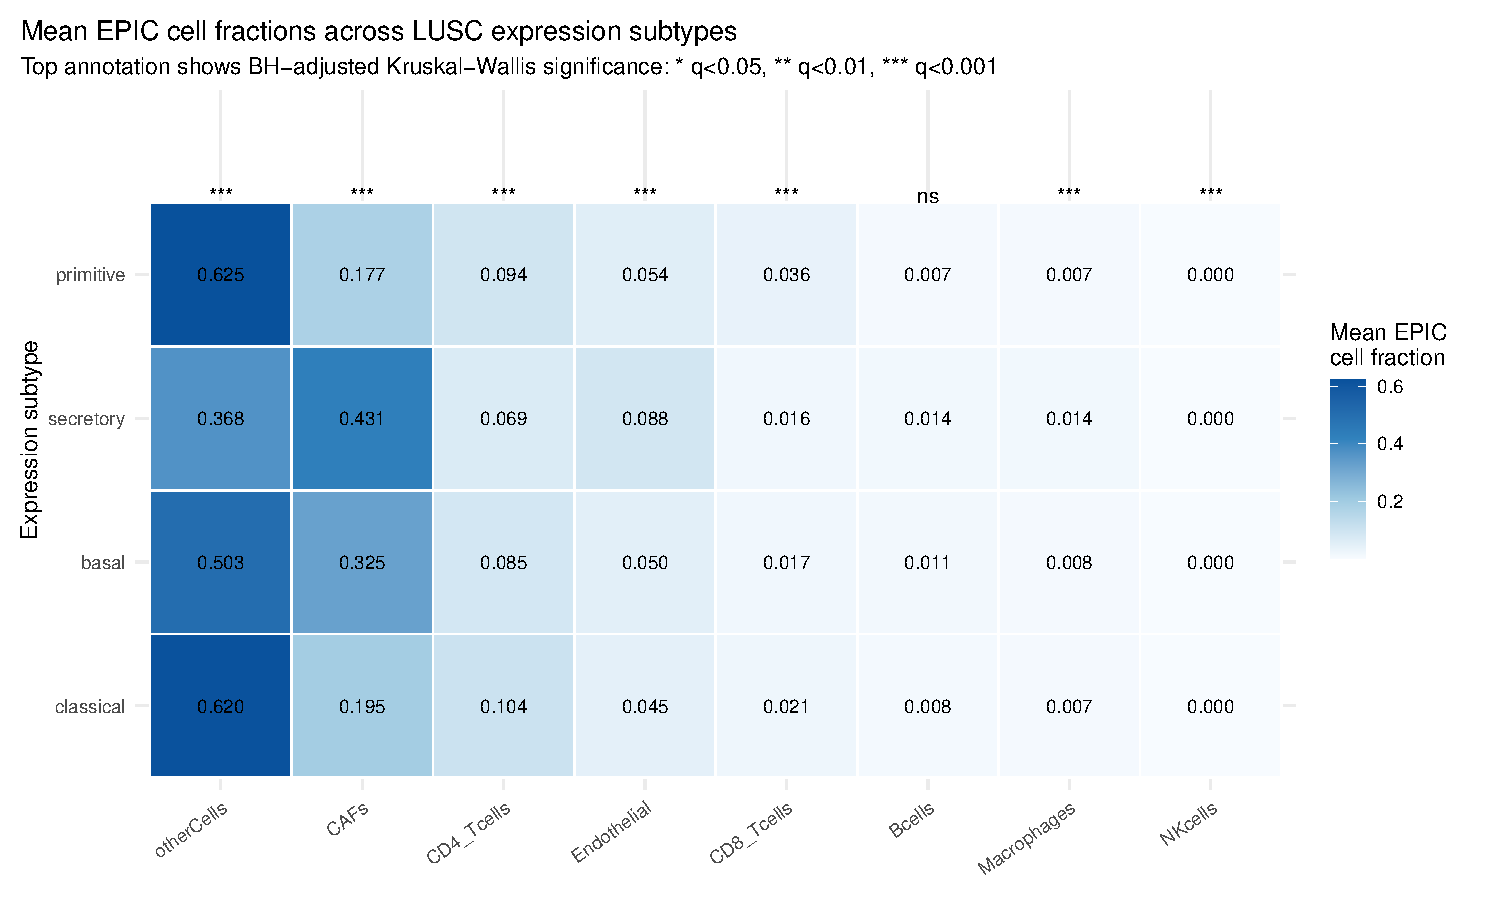
\includegraphics[width=\textwidth]{figures/tme/EPIC_mean_cell_fraction_heatmap.pdf}
    \caption[EPIC immune deconvolution comparison across LUSC subtypes]{
    Mean EPIC cell fractions across LUSC subtypes ($n = 178$). Rows represent expression subtypes; columns represent EPIC-inferred cell compartments ordered by mean fraction. Numeric values show the mean fraction per subtype-cell-type combination. Significance annotations denote BH-adjusted Kruskal-Wallis $q$-values across subtypes ($*q < 0.05$, $**q < 0.01$, $***q < 0.001$; ns: not significant).
    }
    \label{fig:epic_immune_heatmap}
\end{figure}

% TODO: consistent with highly proliferative phenotype -> sounds like it needs a claim.
Secretory subtype showed the highest EPIC fractions for macrophages and CAFs;  primitive subtype showed the highest fraction of uncharacterised cells (otherCells), consistent with its highly proliferative phenotype. B cells did not differ significantly across subtypes.


\begin{figure}[H]
    \centering
    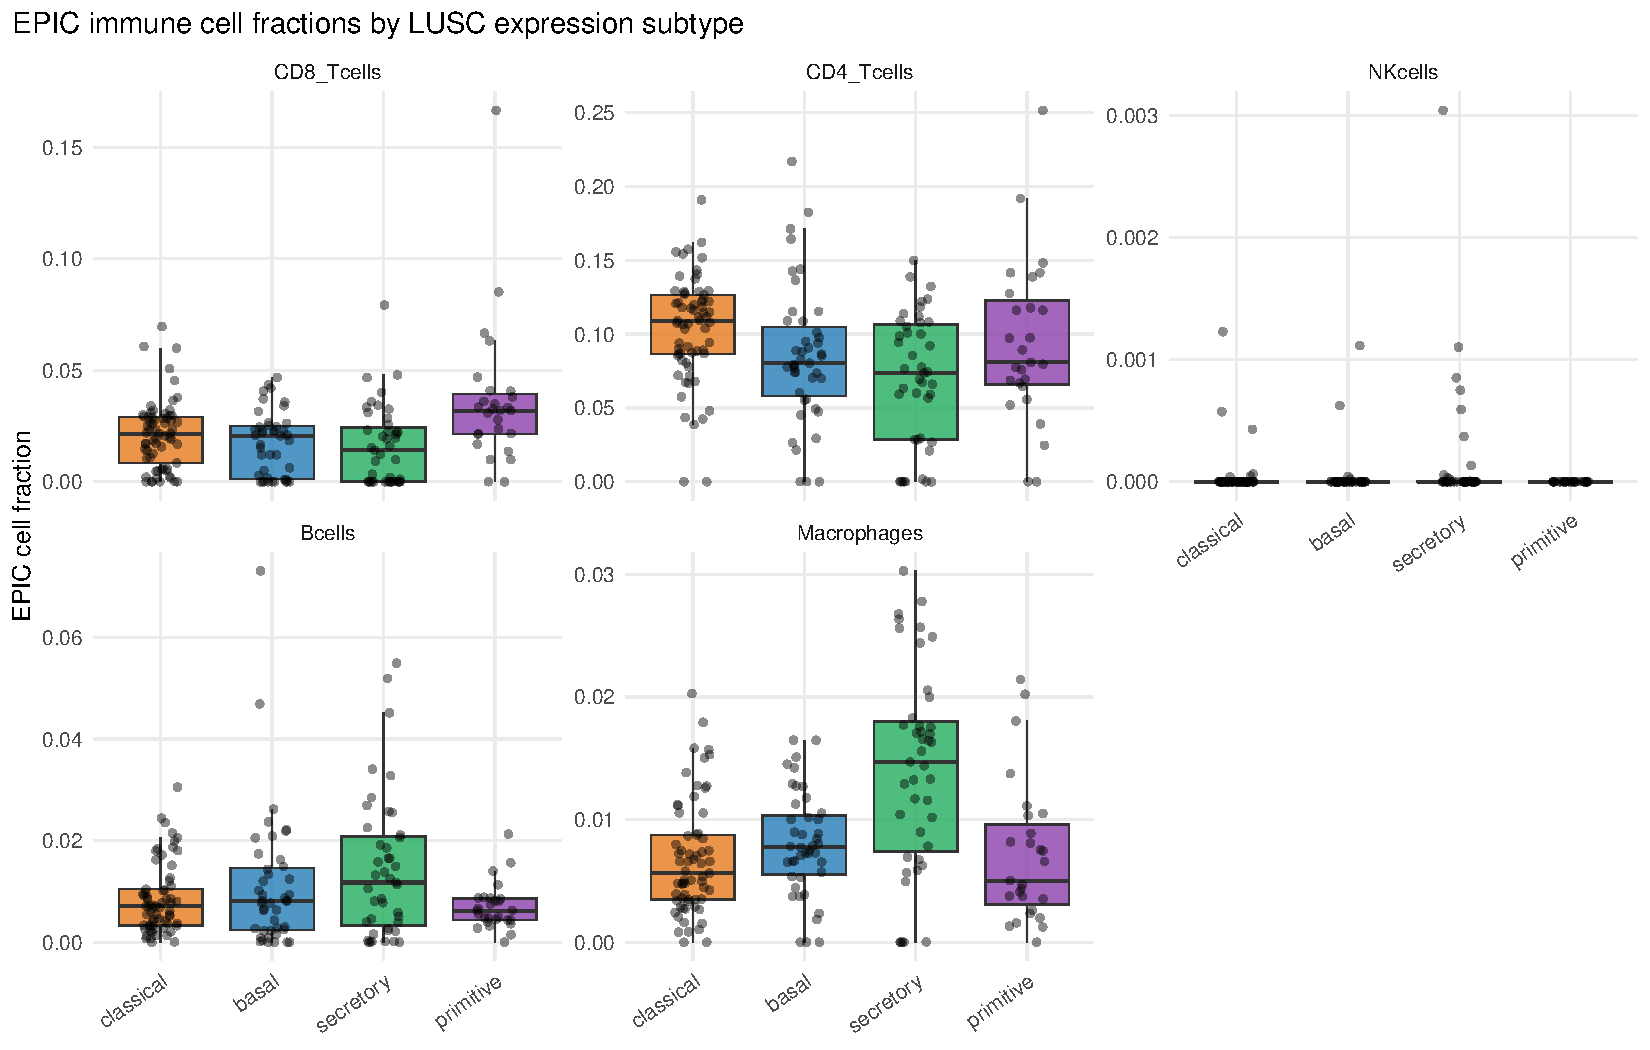
\includegraphics[width=\textwidth]{figures/tme/EPIC_selected_cell_type_boxplots.pdf}
    \caption[EPIC immune cell fractions for selected populations]{
    EPIC-estimated fractions for five cell populations across subtypes. Boxplots show median and interquartile range; individual points are samples. 
    }
    \label{fig:epic_immune_boxplots}
\end{figure}

% Macrophage fractions were highest in the secretory subtype (mean 0.0141) and significantly higher relative to all other subtypes after BH correction. EPIC CD8 T cell fractions were highest in primitive tumours; the discordance with xCell CD8 T cell enrichment scores is discussed in Section~\ref{sec:discussion}.


\begin{figure}[H]
    \centering
    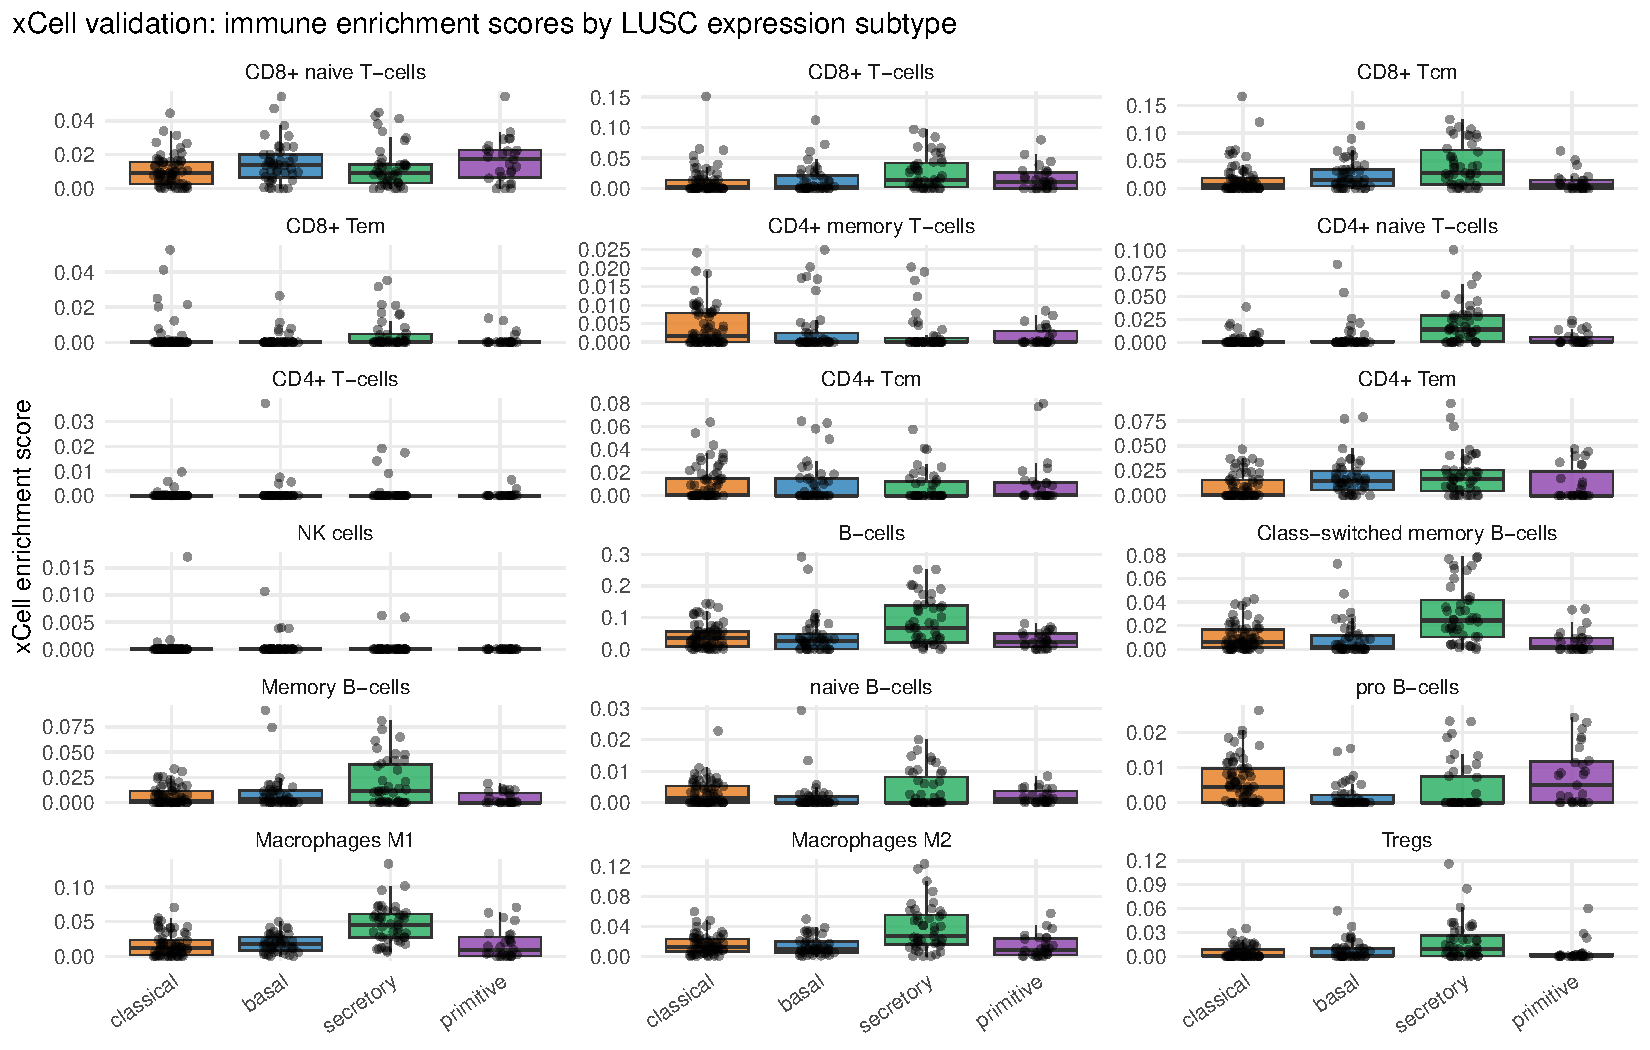
\includegraphics[width=\textwidth]{figures/tme/xCell_selected_cell_type_boxplots.pdf}
    \caption[xCell validation of immune enrichment scores]{
    xCell enrichment scores for selected immune populations across subtypes. xCell scores are relative enrichment estimates, not cell fractions; scores across cell types are not directly comparable. 
    }
    \label{fig:xcell_immune_validation}
\end{figure}

% The secretory subtype showed the highest enrichment for macrophages M1 and M2, B cells, class-switched memory B cells, CD8$^+$ T cells, CD8$^+$ central memory T cells, and Tregs (all $q < 0.05$ after BH correction). Broad NK cell scores did not differ significantly by xCell ($q = 0.642$).
   

\subsection{Somatic Mutation Landscape} %maftools
\label{subsec:somatic_mutation}

\begin{figure}[H]
\centering
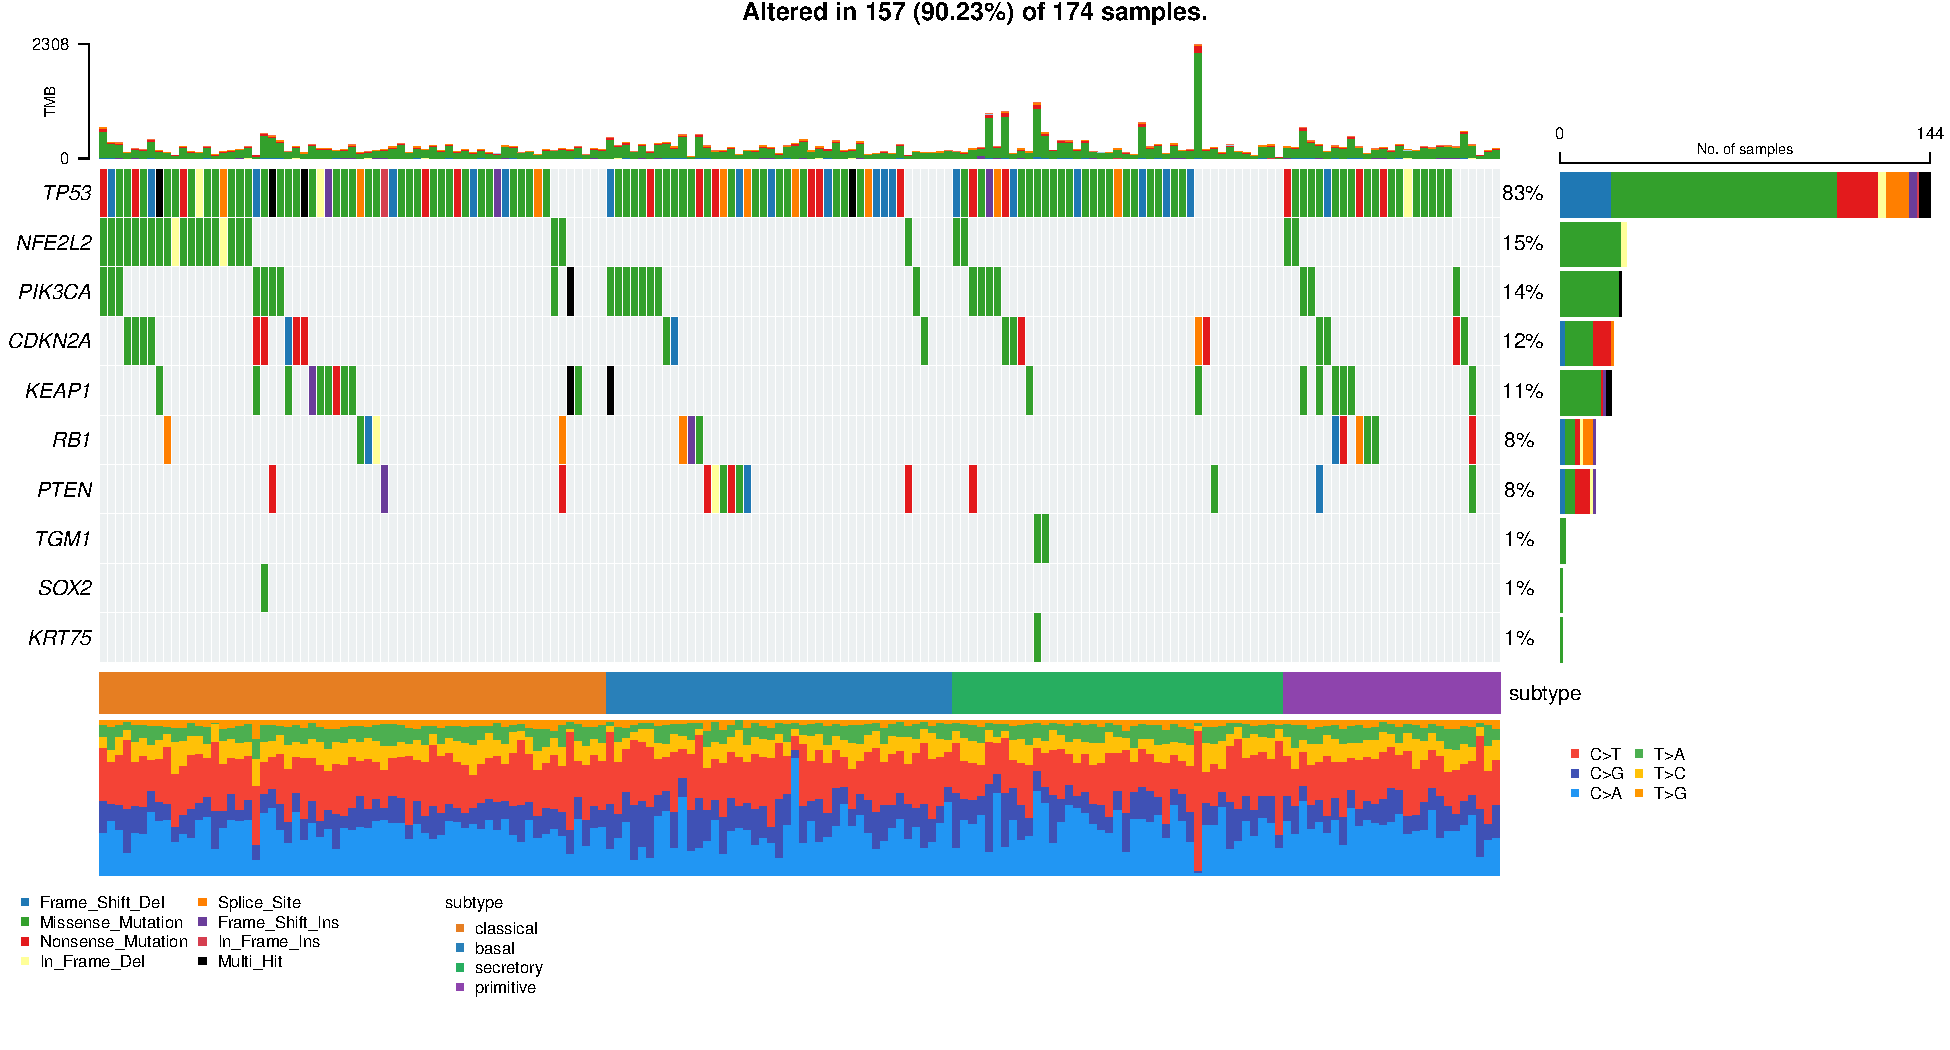
\includegraphics[width=0.98\textwidth]{figures/mutation_analysis/oncoplot_drivers_subtype_annotated.pdf}
\caption[Subtype-annotated oncoplot]{Oncoplot showing gene alterations across subtypes. Curated driver panel consisted of TP53, NFE2L2, KEAP1, RB1, PTEN, CDKN2A, PIK3CA, SOX2, FGFR1, TGM1 and KRT75.}
\label{fig:oncoplot_drivers_subtype_annotated}
\end{figure}


% TODO: it seems i forgot to do pairwise tests; also have to add significance tests to this figure.
TP53 was the most frequently mutated gene overall (Figure~\ref{fig:oncoplot_drivers_subtype_annotated}) but did not show subtype-specific enrichment, consistent with its role as a common subtype-independent driver alteration in LUSC.

\begin{figure}[H]
\centering
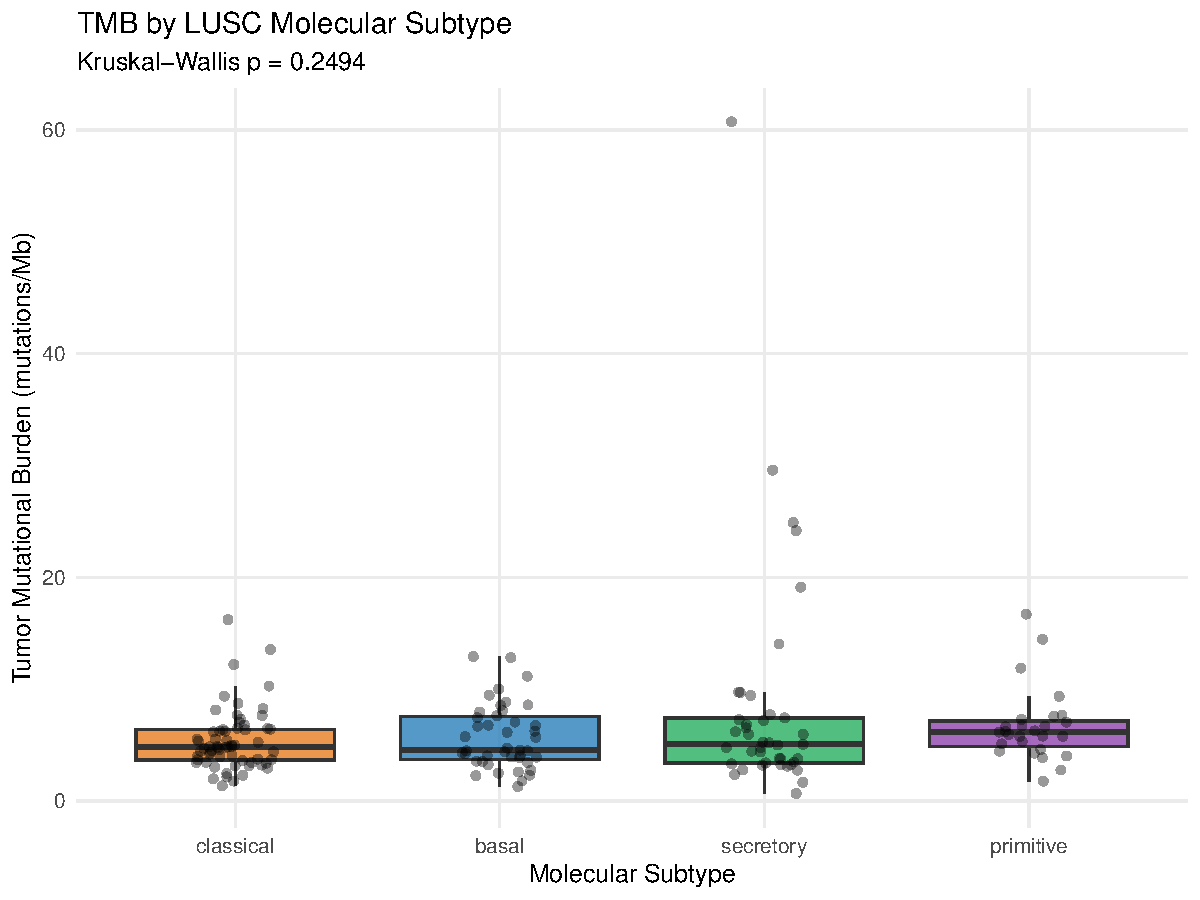
\includegraphics[width=0.65\textwidth]{figures/mutation_analysis/tmb_by_subtype.pdf}
\caption[Tumor mutational burden by subtype]{Tumour mutational burden by subtype.}
\label{fig:tmb_by_subtype}
\end{figure}

TMB did not vary significantly across subtypes (Figure~\ref{fig:tmb_by_subtype}).

\section{Dimensionality Structure and Subtype Separability} 
\label{sec:dim_structure_separability}
% TODO: BE CAREFUL NOT TO CALL THIS VALIDATION OR KEEP WITH VALIDATION STEPS; ITS CHARACTERISATION AT BEST; MAYBE ADD PERMANOVA; MAKES SENSE HERE; SILHOUETTE ON 80% COMPONENTS MAKES MORE SENSE?
%  to show that data isn't noise and subtypes are separable in unsupervised space for a classifier; or is the data noise ;) silhouette score seems to be an easy way to show this. pca for labeled ge samples seems consistent; hard to classify.
%pca+silhouette score, 5 panels; maybe move this to dataset characteristics?
% i think i did pca for ge on kaggle, https://www.kaggle.com/code/rizann/lusc-ge-pca 
% have to check; and get figures with the color palette ive used here.

PCA-based separability analysis revealed substantial differences in subtype structure across omics modalities (Table~\ref{tab:dataset_sep_summary}). 

% TODO: out of ideas; add interpretation later.

\subsection{Dimensionality Structure}

\begin{table}[H]
\footnotesize
\caption[\textcolor{red}{AVOCADO}]{\textcolor{red}{AVOCADO}. PCs denotes the number of components required to represent 80\% of the variance. S denotes Silhouette score. pseudo-F and p denote \gls{permanova} pseudo-F statistic and permutation p-value respectively.}

\centering
\setlength{\tabcolsep}{3pt}
\begin{tabular}{lccccccc}
    \toprule
    \textbf{Modality} & \textbf{n} & \textbf{Features} & \textbf{PCs} & \textbf{PC1(\%)} & \textbf{S} & \textbf{pseudo-F} & \textbf{p} \\
    \midrule
    Gene expression     & 178    & 2000 & 62 & 12.3 & 0.047 & 8.997  & 0.001 \\
    miRNA expression    & 107    & 200  & 30 & 16.6 & 0.031 & 5.191  & 0.001 \\
    RPPA                & 112    & 238  & 27 & 16.4 & 0.008 & 3.935  & 0.001 \\
    DNA methylation     & 76     & 2000 & 11 & 57.7 & -0.060 & 3.491  & 0.005 \\
    CNV                 & 178    & 2000 & 5  & 44.7 & -0.031 & 6.759  & 0.001 \\
    \bottomrule
\end{tabular}
\label{tab:dataset_sep_summary}
\end{table}


The number of principal components required to explain 80\% of cumulative variance varied  across platforms, reflecting differences in feature covariance structure. Gene expression (n=178, 2000 genes) required 62 components, with PC1 explaining 12.3\% of variance. miRNA (n=107, 200 features) required 30 components and RPPA (n=112, 238 proteins) required 27 components. In contrast, methylation (n=76, 2000 probes) reached 80\% variance in only 11 components, with PC1 explaining 57.7\% variance. CNV (n=178, 2000 genes) was the most compact of all modalities, requiring only 5 components with PC1 explaining 44.7\% and PC2 a further 20.8\%.

\subsection{Subtype Separability}

\textbf{\gls{permanova}.} All modalities showed statistically significant subtype group separation (p $\leq$ 0.005), indicating that subtype centroids are non-random across every omics platform. Gene expression showed the strongest centroid separation (pseudo-F = 8.997, p $\leq$ 0.001), followed by CNV (pseudo-F = 6.759, p $\leq$ 0.001), miRNA (pseudo-F = 5.191, p $\leq$ 0.001), RPPA (pseudo-F = 3.935, p $\leq$ 0.001), and methylation (pseudo-F = 3.491, p = 0.005).


% ge:   Per-subtype silhouette: {'classical': 0.0907, 'basal': 0.0697, 'secretory': 0.0248, 'primitive': -0.0621}
% mirna:   Per-subtype silhouette: {'classical': 0.0978, 'basal': 0.0275, 'secretory': 0.006, 'primitive': -0.1334}
% rppa:  Per-subtype silhouette: {'classical': -0.0075, 'basal': 0.0553, 'secretory': 0.0181, 'primitive': -0.0468}
% meth:   Per-subtype silhouette: {'classical': -0.1275, 'basal': -0.0281, 'secretory': -0.0155, 'primitive': -0.0107}
% cnv:   Per-subtype silhouette: {'classical': 0.0872, 'basal': -0.106, 'secretory': -0.0112, 'primitive': -0.2241}

\textbf{Silhouette scores.} Silhouette scores showed remarkable discordance from \gls{permanova}, with gene expression achieving the highest individual-sample cluster cohesion (S = 0.047), followed by miRNA (S = 0.031), RPPA (S = 0.008), CNV (S = -0.031), and methylation (S = -0.060). Negative silhouette scores for CNV and methylation indicate that, on average, samples are geometrically closer to an adjacent subtype's centroid than their own, reflecting high within-group variance relative to between-group separation, even when centroids are statistically distinguishable. 

\textbf{Per-subtype Silhouette scores.} Primitive subtype showed negative mean silhouette scores across all modalities (GE: -0.062; miRNA: -0.133; RPPA: -0.047; methylation: -0.011; CNV: -0.224), indicating that primitive samples are consistently closer to other subtype centroids than to their own. Classical and basal subtypes showed highest silhouette scores across modalities, suggesting more coherent cluster membership in their respective omics feature spaces.

% this finding, that primitive subtypes is kind of what i found in classifier ersults, near-zero per-class F1 for primitive. suggests like: primitive subtype is defined by shared prol. and ep. programs than distinct identity.; maybe address in discussion..

%TODO: add in result: DOES METH HERE SUGGEST a single dominant meth axis, consistent with cpg island methylator phenotype-like structure in luscs?

%DONE: NOW, MAYBE MOVE PER-MODALITY FIGURES TO APPENDIX AND JUST KEEP THE TABLE HERE? chore for future me.

\begin{figure}[H]
\centering
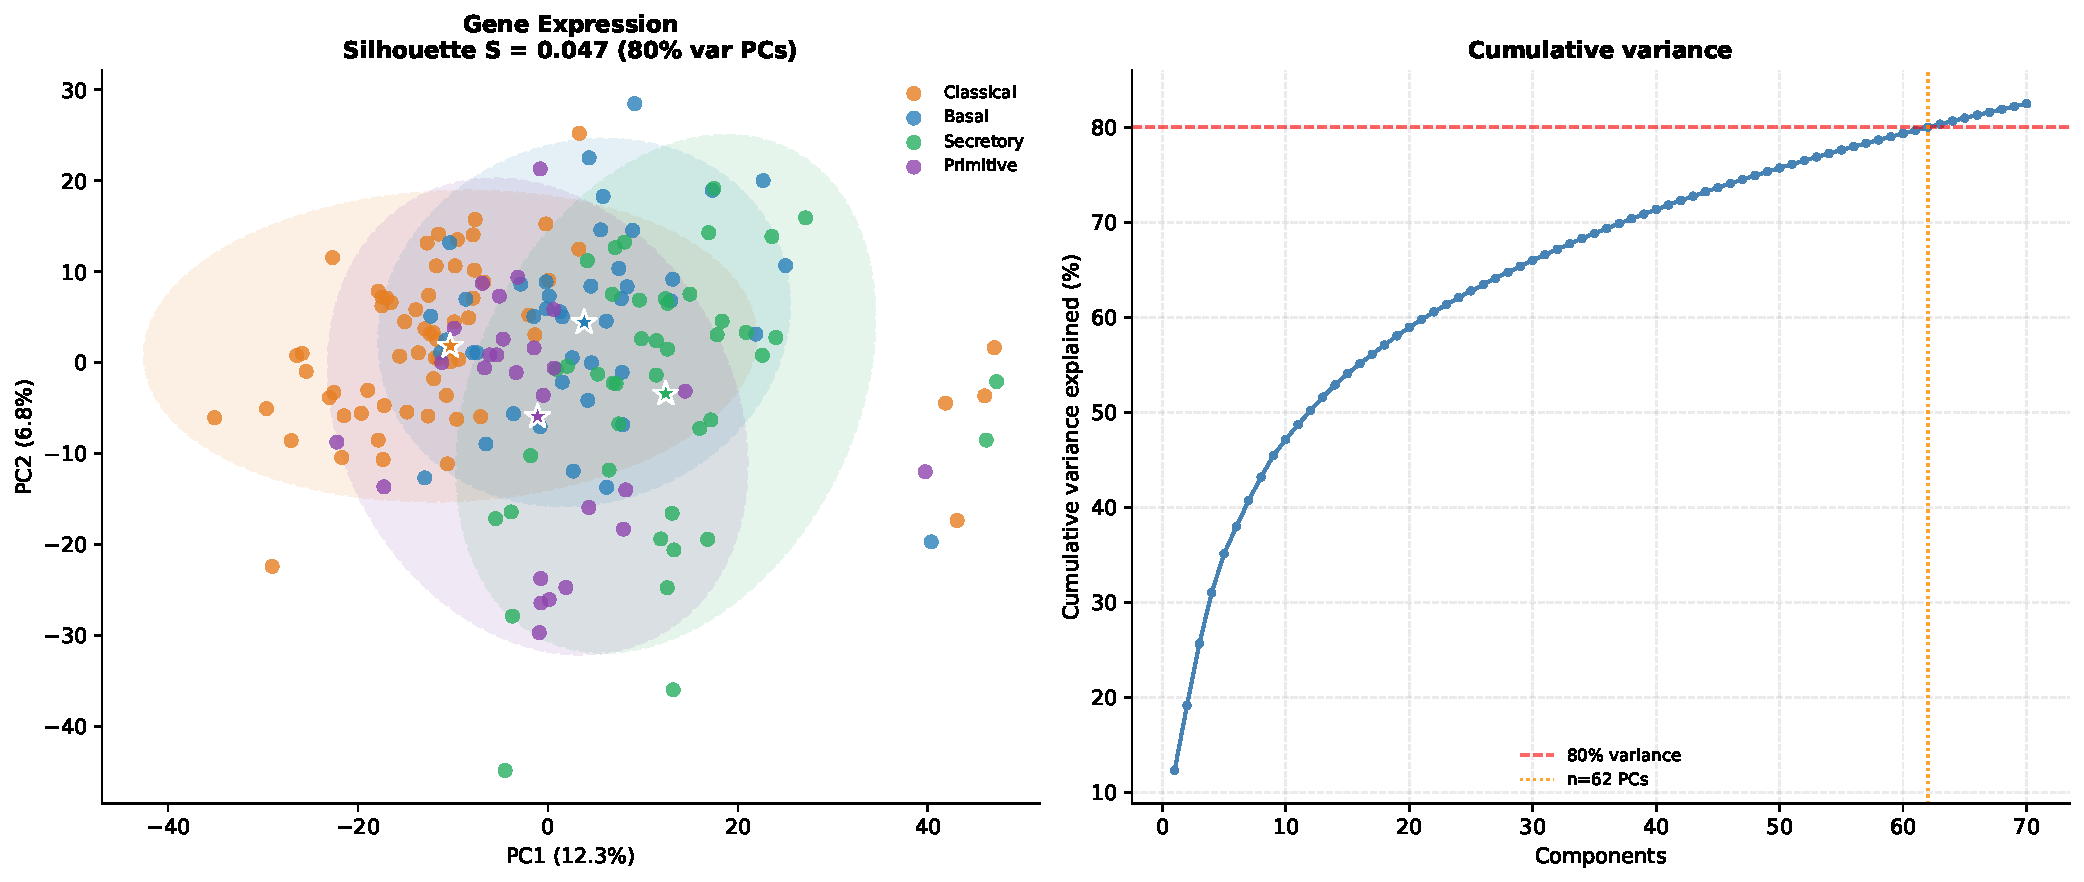
\includegraphics[width=\textwidth]{figures/separability/pca_separability_gene_expression.pdf}
\caption[Principal component analysis of gene expression modality]{Left figure shows PC1 versus PC2 for gene expression; variance explained by each component is shown on the axis label. }
\end{figure}

% Silhouette scores (S) computed on the top-30 principal components represent cluster separation independent of any supervised model.

\begin{figure}[H]
\centering
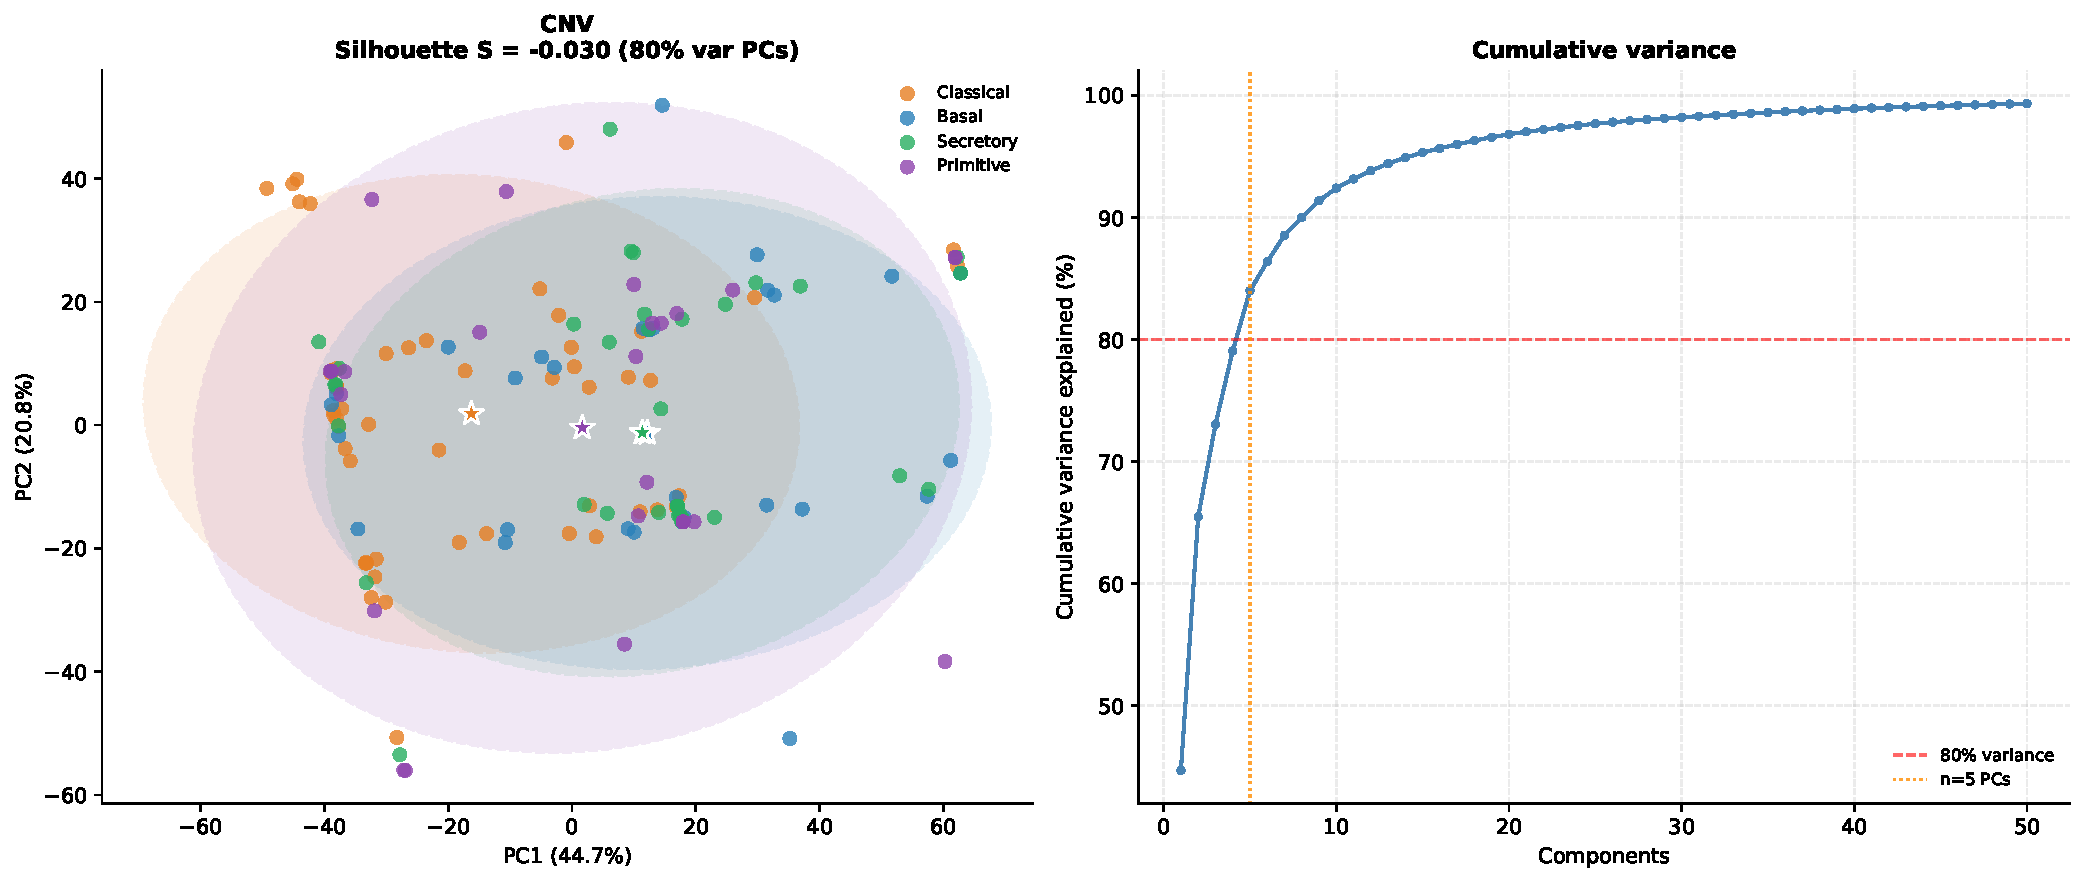
\includegraphics[width=\textwidth]{figures/separability/pca_separability_cnv.pdf}
\caption[Principal component analysis of CNV modality]{Left figure shows PC1 versus PC2 for CNV; variance explained by each component is shown on the axis label. }
\end{figure}

\begin{figure}[H]
\centering
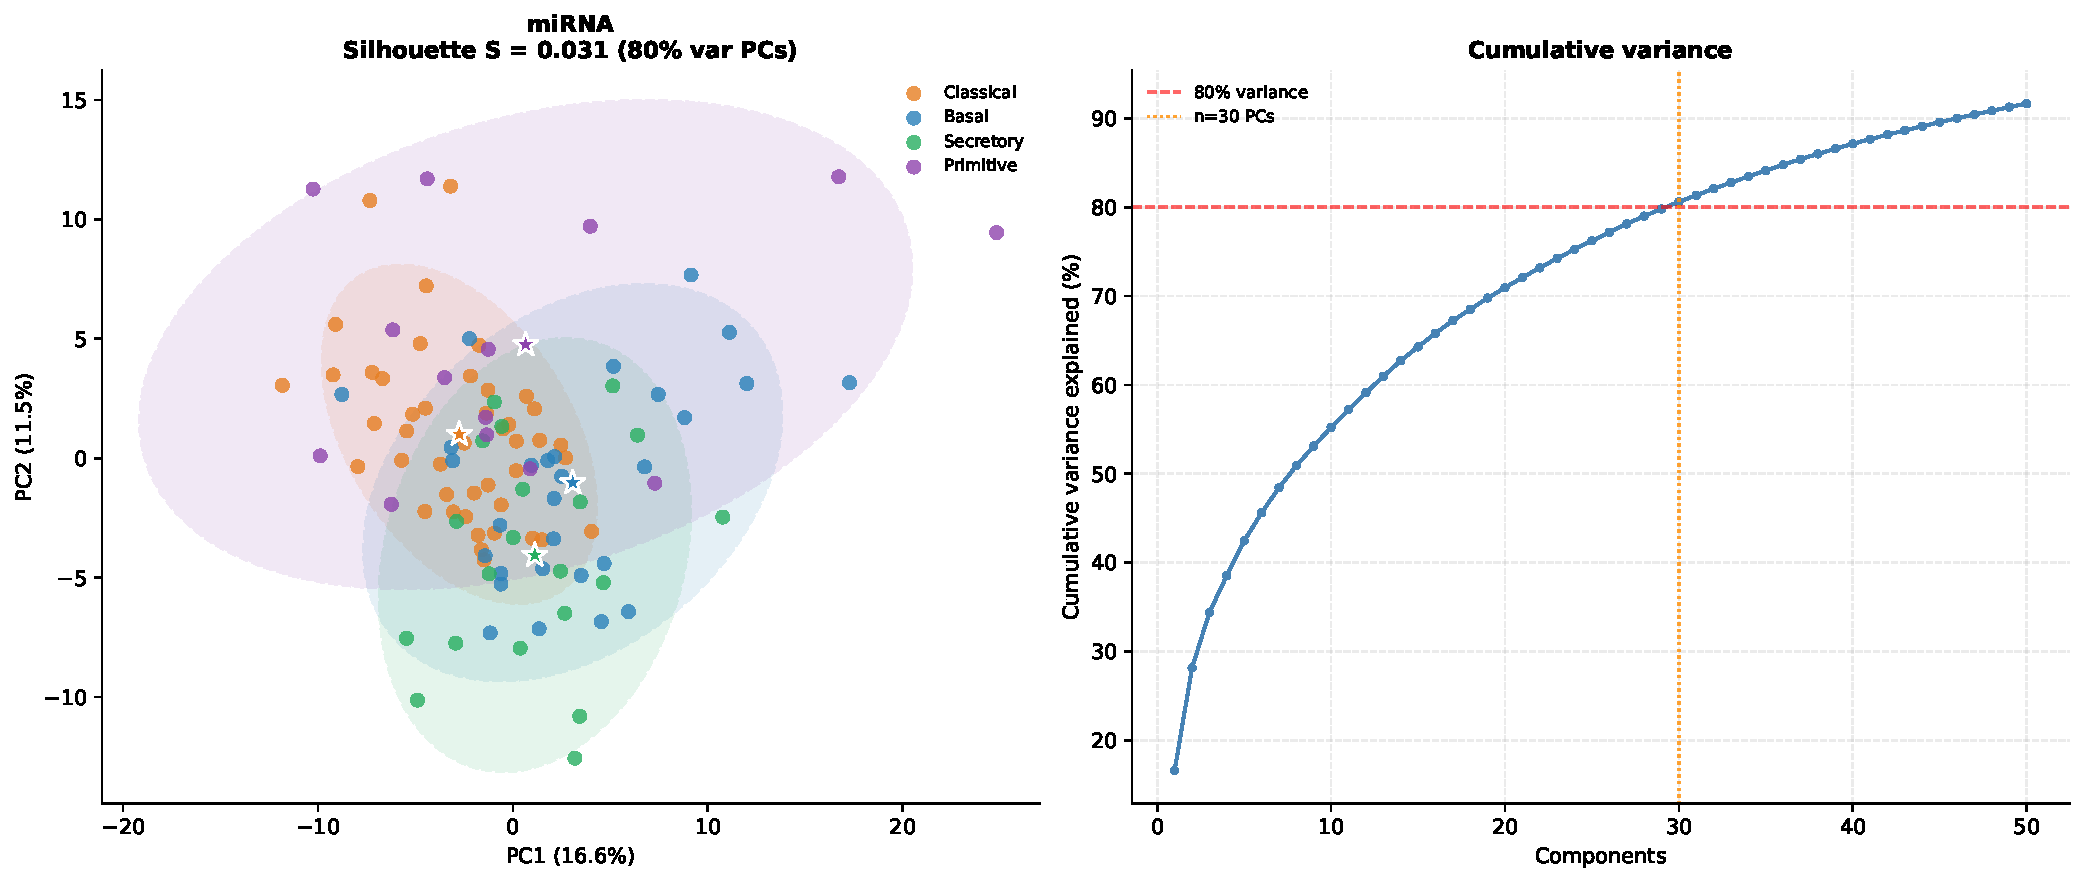
\includegraphics[width=\textwidth]{figures/separability/pca_separability_mirna.pdf}
\caption[Principal component analysis of miRNA modality]{Left figure shows PC1 versus PC2 for miRNA; variance explained by each component is shown on the axis label. }
\end{figure}

\begin{figure}[H]
\centering
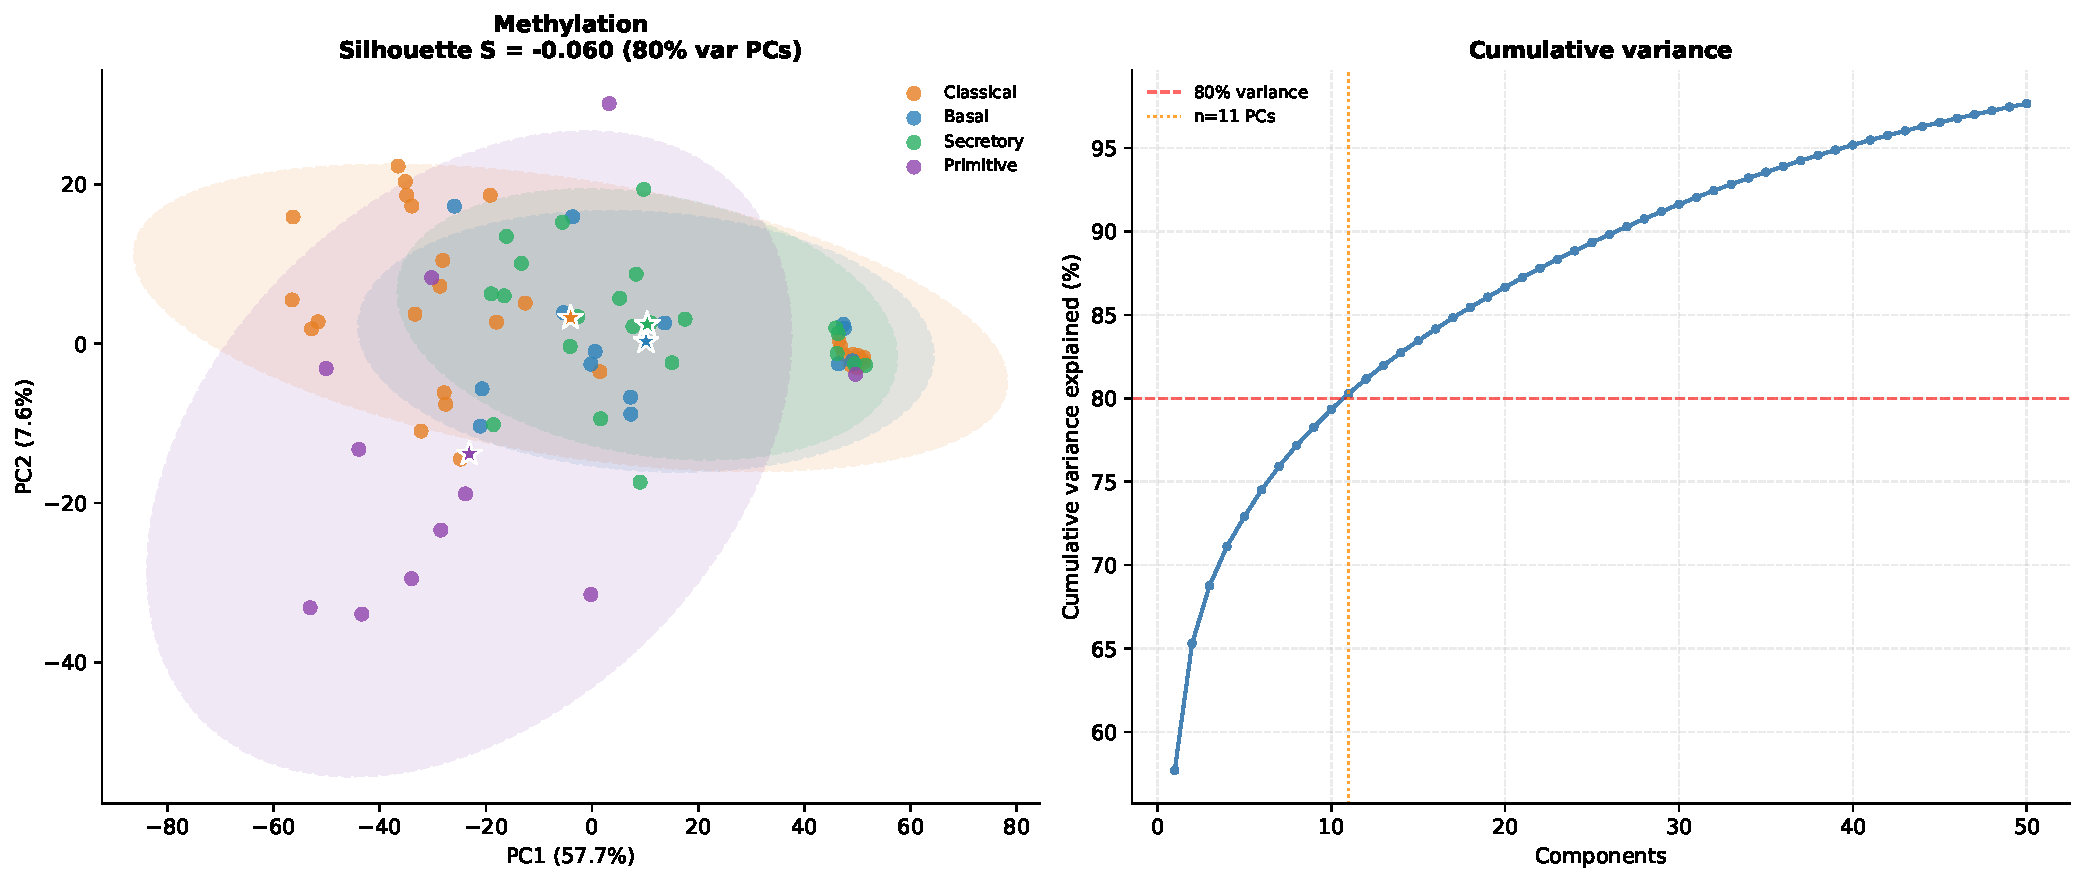
\includegraphics[width=\textwidth]{figures/separability/pca_separability_methylation.pdf}
\caption[Principal component analysis of methylation modality]{Left figure shows PC1 versus PC2 for methylation; variance explained by each component is shown on the axis label. }
\end{figure}

\begin{figure}[H]
\centering
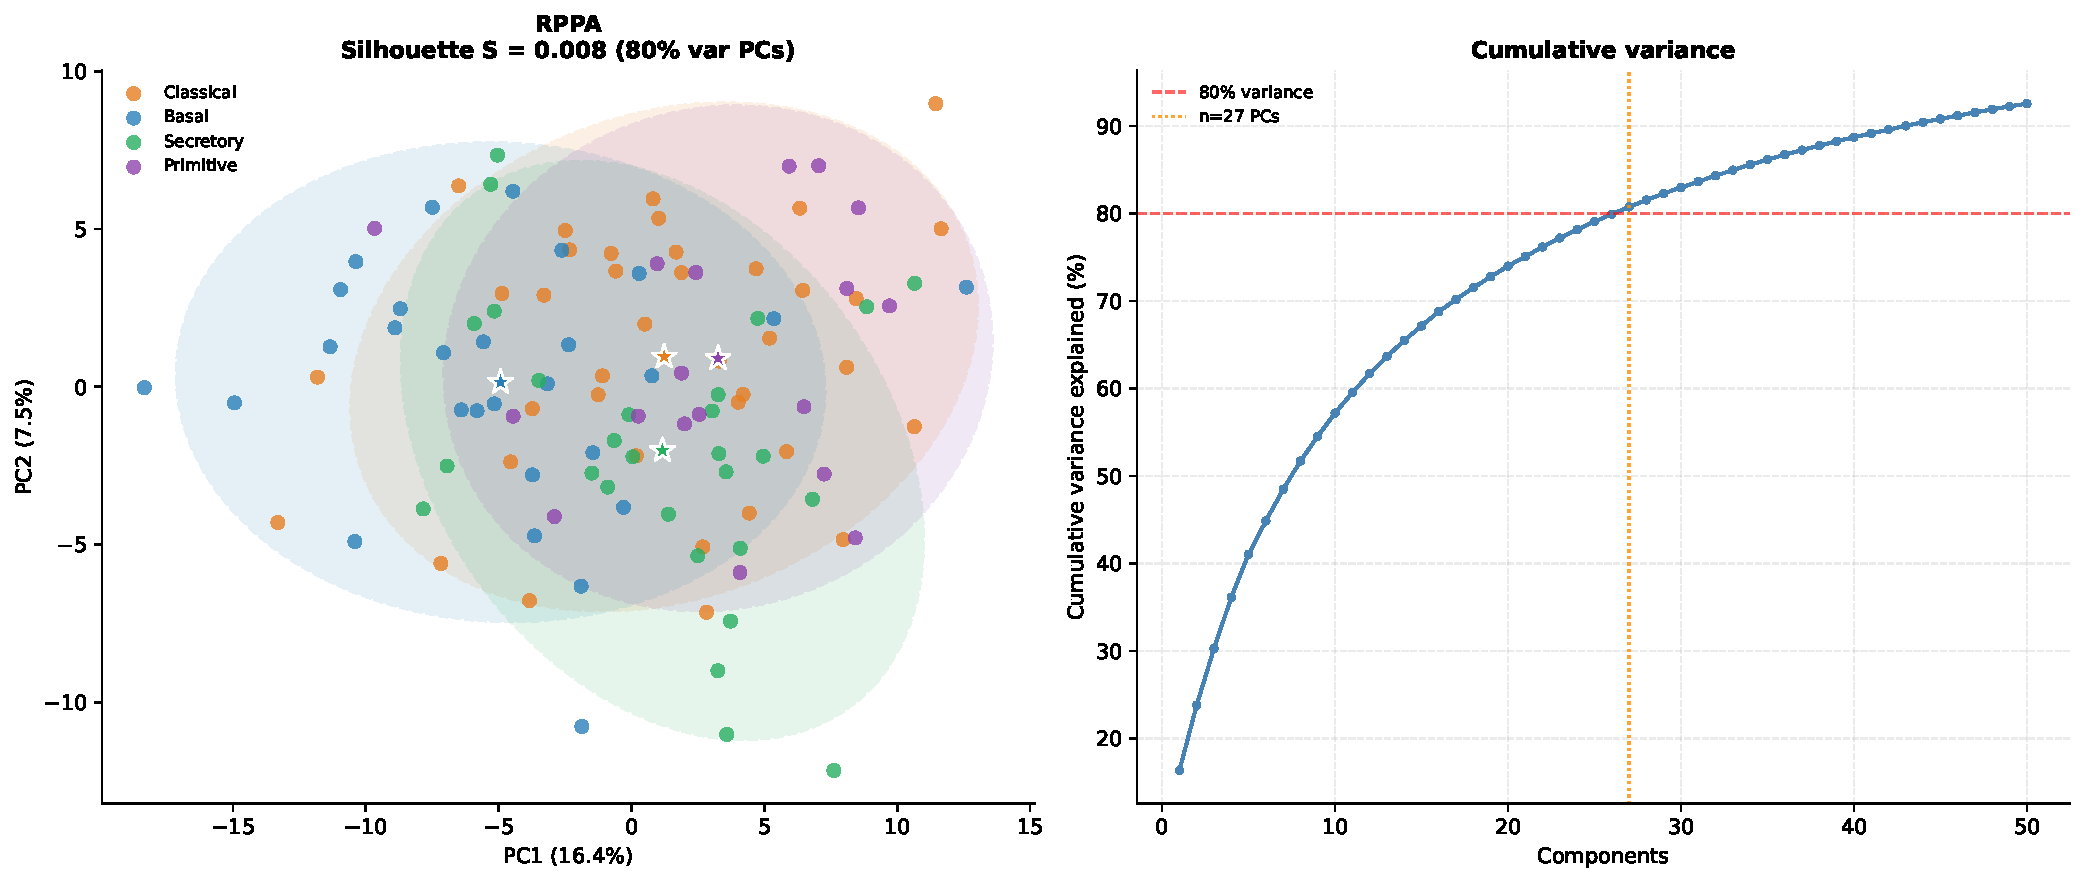
\includegraphics[width=\textwidth]{figures/separability/pca_separability_rppa.pdf}
\caption[Principal component analysis of RPPA modality]{Left figure shows PC1 versus PC2 for RPPA; variance explained by each component is shown on the axis label. }
\end{figure}



\section{Performance Across Omics Modalities}
\label{subsec:omics_perf}

\section{SHAP Feature Importance and Stability}

% pairwise-jaccard similarity
\section{Cross-Model Feature Overlap}

\section{Cross-Modality Feature Overlap}

\section{Pathway Enrichment}

